\section{Correctness audits and performance experiments}
\label{sec:experiments}

The evidence supports a substantial improvement in the ray disc-count query.
It also shows that minimizing transported coordinate bits does not guarantee
a faster complete census.  This section reports both outcomes.  All numbers
are generated from the retained JSON records; the scripts, raw samples,
certificates, input vectors, and SHA-256 source manifests accompany the article.

\subsection{Correctness against an independent geometric implementation}

The corpus contains 48 validated triangulations and 1,801 supplied standard
vertex vectors drawn from the pinned incoming support-kernel corpus.  We
augment these with zero vectors and deterministic compatible positive
combinations, removing duplicates within each triangulation.  The resulting
2,980 sources include layered solid tori, boundary caps, interior vertices,
Pachner-modified examples, trefoil and figure-eight exteriors, and solid-torus
connected sums with $\mathbb{RP}^3$ and $S^2\times S^1$.

For every source the audit compares the maintained full-coordinate census,
the new vector observer, and its packed realization.  It independently
replays both new profile certificates and the ray-block disc certificate.
It also constructs the actual connected components in Regina~7.4, compares
their full vectors and multiplicities, and uses Regina's compressing-disc
test on those connected components.  Literal component construction is
restricted to these small audit inputs; the huge scaling tests never expand
normal sheets.

\begin{center}
\begin{tabular}{@{}lr@{}}
\toprule
Audit item & Result \\
\midrule
Triangulations & 48\\
Supplied normal sources & 2,980\\
New/baseline result comparisons & 8,940 agreements\\
Independent certificate replays & 8,940 accepted\\
Regina full-profile and disc-count comparisons & 2,980 agreements\\
Deliberately mutated profile proofs & 27 rejected\\
Focused new and affected regression tests & 146 passed\\
Additional exact rational matrix audit & 40 systems, 420 bases\\
\bottomrule
\end{tabular}
\end{center}

The nullity distribution is $48,2091,524,217,90,8,2$ sources for
$d=0,1,2,3,4,5,6$, respectively.  Among 2,932 nonempty sources, 2,117 are
settled entirely by ray blocks.  Across all sources, 1,644 blocks use peeling,
499 use the generic rank-one certificate, and 815 invoke the complete fallback.
These are coverage counts for this constructed, vertex-vector-heavy corpus,
not estimates for arbitrary knot diagrams.  Both profile inequalities and the
identical vector/packed run statistics hold on every audited source.

The 146-test focused suite contains 42 new test methods and 104 affected
maintained tests.  All pass without skips in the recorded Regina-enabled run.
The suite covers the code changed by this additive package and its mathematical
dependencies; it is not represented as a rerun of every historical research
test in the repository.  A separate dense rational oracle checks the greedy
minimum against exhaustive eligible bases on 40 small integer systems,
independently of the producer's fraction-free and checker's modular methods.
The unit tests add 100 randomized exhaustive comparisons.

Adversarial checks alter ranks, minor rows, kernel entries, denominators,
supports, scalar weights, component multiplicities, primitive divisors,
boundary parities, sources, and schema fields.  They exercise valid composite
moduli with unit pivots and reject invalid nonunit pivots.  Several tests
disable producer functions during verification.  One-sided M\"obius bands,
closed projective planes, source vectors with more than 20,000-bit common
multiplicity, exact hexadecimal transport, and callback identity propagation
target failure modes that ordinary meridian examples would miss.

\subsection{Timing protocol and reproducibility limits}

The final run uses CPython~3.12.14 on Linux x86-64, with garbage collection
enabled.  Each arm has one retained warm-up followed by five paired rounds;
larger cohorts use three.  An initially seeded shuffled order is reversed in
the next round.  A/A arms run the same implementation twice under distinct
labels to expose timing variation.  Inputs, JSON serialization, result
comparison, and artifact writing are outside the timed region.

Every timed public query includes fresh source validation, certificate
generation, and one separately timed independent external verification.  The
new ray producer also performs its own internal replay, which remains inside
generation time.  Thus its reported time includes \emph{more} replay than
the old disc producer; no cost is subtracted to equalize this implementation
choice.  The source-bound wrapper includes two internal disc replays and a
further timed external source-bound replay.  A sampled cancellation/time-limit
callback is active in every arm; its cost is included.

The run completes 27 cohorts and 652 calls: 538 measured and 114 warm-up
calls.  There are no timeouts, errors, or budget skips, and all source hashes
match before and after.  The protocol predeclares the omission of old-query
comparisons at 512 tetrahedra; that size is only a new-ray capacity and A/A
case.  The timeout limits are retained in the script for reproducibility,
not used to censor any measured pair.

Each reported speedup is the median of the within-round old/new ratios.
The time columns are medians computed separately for each arm, so their
quotient need not equal the paired median ratio.  Ratios above one favour the
new method.  Across all A/A controls the median-ratio range is
$0.862928$--$1.093790$.  Small differences within this range should not be
treated as robust improvements, and three large-case rounds do not supply
a general statistical confidence interval.  Measurements are single-host
observations with recorded instrumentation, not universal hardware constants.

% Automatically generated from the retained benchmark; do not hand-edit numerical rows.
Table entries are separate medians in milliseconds. Each ratio is the median
of the first time divided by the second time within the same measured round;
it need not equal the ratio of the two displayed medians. Warm-ups are excluded.

\begin{table}[tbp]
\centering\small
\setlength{\tabcolsep}{4.5pt}
\caption{Fibonacci meridian disc counts. Both methods include fresh generation and one external replay; the ray producer also performs its existing internal replay. The 512-tetrahedron entry is a ray-only capacity measurement, with no baseline ratio.}
\label{tab:raytimes}
\begin{tabular}{rrrrr}
\toprule
$t$ & Pairs/calls & Old disc (ms) & Ray disc (ms) & Old/ray \\
\midrule
8 & 5 & 3.603 & 2.428 & 1.484 \\
16 & 5 & 8.400 & 4.597 & 1.830 \\
32 & 5 & 23.453 & 8.409 & 2.733 \\
64 & 5 & 82.226 & 19.655 & 4.279 \\
128 & 5 & 282.173 & 36.260 & 7.524 \\
256 & 3 & 1351.121 & 72.965 & 18.704 \\
512 & 3 & --- & 227.015 & --- \\
\bottomrule
\end{tabular}
\end{table}

\begin{table}[tbp]
\centering\small
\setlength{\tabcolsep}{4.5pt}
\caption{Complete coordinate censuses on the same Fibonacci sources: dimension reduction does not compensate for general rank-compilation overhead in this experiment. The old implementation already uses its single-orbit shortcut. There are five pairs through $t=128$ and three at $t=256$.}
\label{tab:coordinatetimes}
\begin{tabular}{rrrrrrr}
\toprule
$t$ & $q+a$ & $d$ & Old (ms) & $d$-vector (ms) & Packed (ms) & Old/packed \\
\midrule
8 & 8 & 1 & 2.938 & 3.130 & 3.143 & 0.916 \\
16 & 16 & 1 & 7.163 & 8.576 & 8.176 & 0.868 \\
32 & 32 & 1 & 22.625 & 26.072 & 26.098 & 0.867 \\
64 & 64 & 1 & 79.959 & 97.105 & 93.013 & 0.855 \\
128 & 128 & 1 & 288.641 & 368.977 & 347.524 & 0.820 \\
256 & 256 & 1 & 1335.527 & 1445.574 & 1707.417 & 0.782 \\
\bottomrule
\end{tabular}
\end{table}

\begin{table}[tbp]
\centering\small
\setlength{\tabcolsep}{4.5pt}
\caption{Control cases, five pairs per row. The first and second methods are named in each group heading. Fixed-trace transport uses an identical selected basis and independently checked orbit trace in both arms; its excluded setup contains geometry, compilation, weight construction, and orbit discovery.}
\label{tab:controls}
\begin{tabular}{lrrr}
\toprule
Case & First (ms) & Second (ms) & First/second \\
\midrule
\multicolumn{4}{l}{\emph{Disc counts: old kernel / ray interface}} \\
Vertex links & 0.398 & 1.515 & 0.259 \\
Three-way mixture & 1.394 & 3.323 & 0.416 \\
Capped meridian & 5.568 & 15.471 & 0.346 \\
\addlinespace[3pt]
\multicolumn{4}{l}{\emph{Coordinate censuses: old compact / packed}} \\
Vertex links & 2.381 & 2.551 & 0.920 \\
Three-way mixture & 2.873 & 3.356 & 0.917 \\
Capped meridian & 18.637 & 16.711 & 1.087 \\
\addlinespace[3pt]
\multicolumn{4}{l}{\emph{Fixed-trace transport: vector / packed}} \\
Vertex links & 0.886 & 0.914 & 0.953 \\
Three-way mixture & 1.003 & 1.059 & 1.004 \\
Capped meridian & 9.502 & 9.199 & 1.042 \\
\bottomrule
\end{tabular}
\end{table}

\begin{table}[tbp]
\centering\small
\setlength{\tabcolsep}{4.5pt}
\caption{Source-bound certificates for stabilized-circle diagrams. The existing cocycle discovers the supplied vector outside the timers. Generation includes two internal disc replays, followed by a separately timed external source-bound replay. These are new-wrapper A/A stages, not a comparison of complete automatic recognizers. Separate stage medians need not sum to the total median.}
\label{tab:diagramtimes}
\begin{tabular}{rrrrrrr}
\toprule
Crossings & $t$ & Calls & Generate (ms) & Verify (ms) & Total (ms) & Proof bytes \\
\midrule
1 & 20 & 5 & 8.072 & 2.878 & 11.023 & 4,283 \\
4 & 80 & 5 & 24.331 & 8.686 & 34.129 & 16,333 \\
8 & 160 & 5 & 54.233 & 17.607 & 70.303 & 32,823 \\
16 & 320 & 3 & 111.712 & 45.605 & 159.955 & 66,815 \\
32 & 640 & 3 & 255.049 & 81.645 & 342.695 & 134,943 \\
\bottomrule
\end{tabular}
\end{table}



\subsection{The successful specialization: disc counts on Fibonacci rays}

\Cref{tab:raytimes} reports the principal gain.  At 256 tetrahedra, the old
disc query has median total time $1351.121$ ms and the peeled query has median
$72.965$ ms.  The paired median improvement is $18.704$ times, with paired
range $17.083$--$20.191$ in the three rounds.  The new method establishes the
single supported ray and its primitive disc data directly; it avoids the
orbit discovery that the old primitive-core query still performs.

At that size the serialized disc certificate shrinks from 7,098,789 to
15,368 bytes, about a factor of 462.  Both sizes use the same compact JSON
serialization and exclude the separately stored source input.  The old
certificate records 261 orbit cycles and 81,930 transmissions, while the new
one records one peeling block and zero orbit cycles.  These counters explain
the measured difference without turning an observed scheduling pattern into
a theorem about all interval algorithms.

At 512 tetrahedra the new query has median total time $227.015$ ms and a
32,264-byte certificate.  This establishes tested capacity on that input;
it has no measured old/new ratio.  The all-family asymptotic statement comes
from \cref{thm:fibonacci}, whose $3t-1$ steps are proved for every $t$ and
every positive integer multiplier, independently of these timing samples.

\begin{figure}[tbp]
\centering
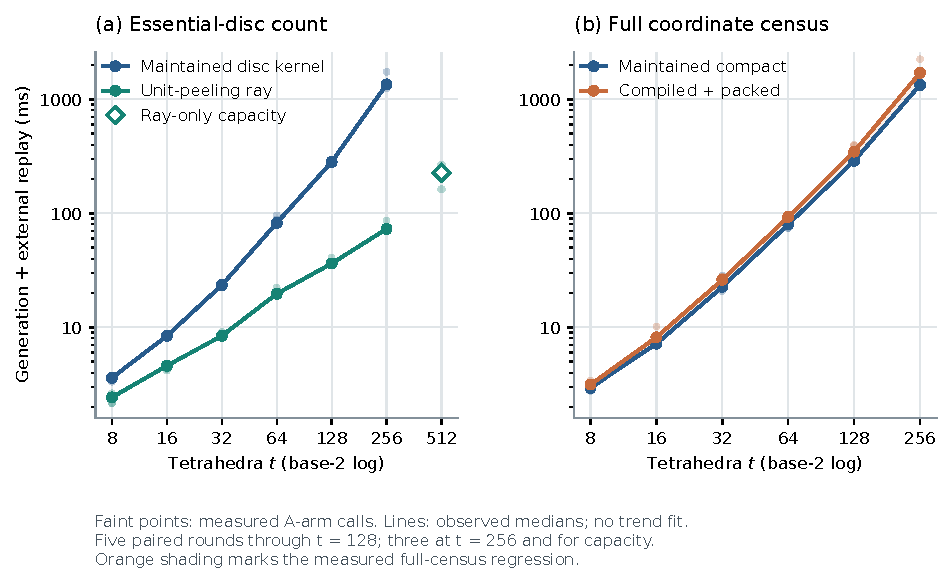
\includegraphics[width=\linewidth]{benchmarks.pdf}
\caption{Recorded generation plus independent external verification times.
The ray-disc specialization improves strongly on this family; the general
packed full-coordinate census does not.  Points are measured medians, with
no fitted asymptotic curve.  The new-ray-only 512-tetrahedron point is a
capacity measurement.}
\label{fig:benchmarks}
\end{figure}

\begin{figure}[tbp]
\centering
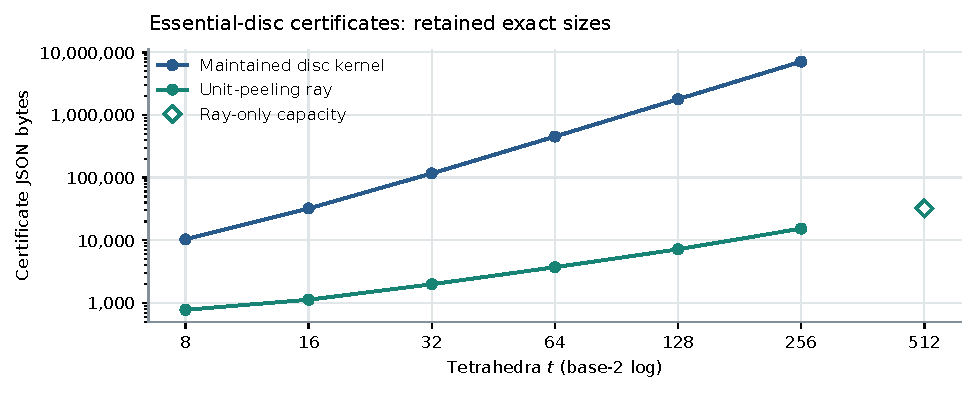
\includegraphics[width=0.88\linewidth]{proof_sizes.pdf}
\caption{Compact JSON disc-certificate sizes on the same family, excluding
source input.  The independently replayable unit-row transcript avoids the
large retained orbit trace.  The 512-tetrahedron diamond has no old-query
comparison; connecting lines only link measured values.}
\label{fig:proofsizes}
\end{figure}

\subsection{Negative and inconclusive performance findings}

\Cref{tab:coordinatetimes} is an essential qualification.  On the same
Fibonacci family the general packed census is slower at every measured size.
At $t=256$ the old census takes median $1335.527$ ms and the packed census
$1707.417$ ms, with old/new paired ratio $0.782$.  The new projection reduces
dimension from 256 to one, but the baseline already invokes its single-orbit
shortcut for weighted transport.  The common orbit discovery remains, and
general rank compilation adds cost.  A mathematically optimal slot budget
has not become a faster end-to-end query here.

The ray API also regresses on the three overhead controls in
\cref{tab:controls}: interior links, an interior sphere/disc/M\"obius mixture,
and a capped meridian with links.  The old primitive-core routine disposes of
these small cases cheaply.  The new conservative block construction, rank
gate, repeated geometry scans, and internal replay cost more than they save.
This is why the additions are explicit APIs, with no automatic replacement
of the default policy.

The isolated transport comparison holds the selected basis and unweighted
orbit trace fixed.  Vector/packed paired ratios are $0.953$, $1.004$, and
$1.042$ for the three controls.  The last has a broad paired range
$0.632$--$1.701$.  These observations validate the shared-run comparison but
do not establish a robust scalar-packing wall-clock advantage.  The capped
full census gives a small $1.087$ paired improvement, likewise too close to
the A/A variation to motivate a broad default change.

The practical conclusion is specific: the peeled rank-one disc gate is a
demonstrated improvement on the dense tested family.  The general observer
provides exact minimal dimension, optimal allocated bits, reusable rank
evidence, and a foundation for later work; current measurements do not justify
advertising it as a universal acceleration.

\subsection{Source-bound diagram stages}

\Cref{tab:diagramtimes} reports positive braid stabilizations of a circle:
the closure of $\sigma_1\sigma_2\cdots\sigma_n$ on $n+1$ strands.  The
maintained cocycle routine supplies a vector before timing.  The measured
stage constructs the canonical exterior, generates the new positive proof,
and independently checks its source binding.  All sizes through 32 crossings
and 640 exterior tetrahedra complete.  There is an A/A control but no old/new
recognizer comparison.  These inputs verify the source connection of the
new certificate path; they are not evidence that the complete recognizer is
faster on hard unknot diagrams.
